\documentclass[14pt,a4paper]{extarticle}

% Поддержка различных компиляторов (pdfLaTeX, XeLaTeX, LuaLaTeX) на Overleaf
\usepackage{iftex}
\ifPDFTeX
  \usepackage[T2A]{fontenc}
  \usepackage[utf8]{inputenc}
  \usepackage[russian]{babel}
  \usepackage{tempora}
  \usepackage{courier}
\else
  \usepackage{fontspec}
  \defaultfontfeatures{Ligatures=TeX}
  \setmainfont{Times New Roman}
  \setmonofont{Courier New}
  \usepackage{polyglossia}
  \setmainlanguage{russian}
\fi

% Поля страницы по стандарту БГУИР СТП 01-2017 (Приложение Л)
\usepackage[a4paper, left=30mm, right=15mm, top=20mm, bottom=20mm]{geometry}

% Межстрочный интервал 1.5 и абзацный отступ 1.25 см
\usepackage{setspace}
\onehalfspacing
\usepackage{indentfirst}
\setlength{\parindent}{1.25cm}
\setlength{\parskip}{0pt}

% Колонтитулы: номер страницы в нижнем правом углу
\usepackage{fancyhdr}
\pagestyle{fancy}
\fancyhf{}
\renewcommand{\headrulewidth}{0pt}
\fancyfoot[R]{\thepage}
\fancypagestyle{plain}{
  \fancyhf{}
  \fancyfoot[R]{\thepage}
  \renewcommand{\headrulewidth}{0pt}
}

% Оформление заголовков по стандарту СТП 01-2017
\usepackage{titlesec}
\titleformat{\section}[block]{\raggedright\bfseries\fontsize{14pt}{17pt}\selectfont}{\thesection}{1em}{}
\titleformat{\subsection}[block]{\raggedright\bfseries\fontsize{14pt}{17pt}\selectfont}{\thesubsection}{1em}{}
\titlespacing*{\section}{1.25cm}{14pt}{6pt}
\titlespacing*{\subsection}{1.25cm}{10pt}{4pt}

% Настройка подписей к рисункам: «Рисунок X.Y – Название»
\usepackage{graphicx}
\usepackage{caption}
\DeclareCaptionLabelSeparator{dash}{~--~}
\captionsetup[figure]{labelsep=dash, name={Рисунок}, justification=centering, font=normalsize}
\counterwithin{figure}{section}

% Окружение для моноширинного листинга кода без рамок
\usepackage{fvextra}
\DefineVerbatimEnvironment{CodeListing}{Verbatim}{
  fontsize=\fontsize{9pt}{10.5pt}\selectfont,
  breaklines=true,
  breakanywhere=false,
  frame=none,
  numbers=none,
  baselinestretch=1.0
}

\newcommand{\listingtitle}[1]{%
  \par\vspace{8pt}%
  \noindent\hspace*{1.25cm}\textbf{#1}\par\vspace{2pt}%
}

\begin{document}

% =========================================================================
% ТИТУЛЬНЫЙ ЛИСТ (весь текст строго НЕ жирным шрифтом)
% =========================================================================
\begin{titlepage}
\thispagestyle{empty}
\begin{center}
{\fontsize{11pt}{13pt}\selectfont
МИНИСТЕРСТВО ОБРАЗОВАНИЯ РЕСПУБЛИКИ БЕЛАРУСЬ\par
БЕЛОРУССКИЙ ГОСУДАРСТВЕННЫЙ УНИВЕРСИТЕТ\par
ИНФОРМАТИКИ И РАДИОЭЛЕКТРОНИКИ\par
Факультет компьютерных систем и сетей\par
Кафедра программного обеспечения информационных технологий\par}

\vspace{4.5cm}

{\fontsize{16pt}{20pt}\selectfont
ОТЧЕТ\par
ПО ЛАБОРАТОРНОЙ РАБОТЕ № 1\par}

\vspace{0.8cm}

{\fontsize{14pt}{17pt}\selectfont
по дисциплине «Методы машинного обучения»\par\vspace{0.5cm}
Вариант № 7\par}
\end{center}

\vspace{3.2cm}

\begin{flushright}
\begin{minipage}{0.46\textwidth}
{\fontsize{13pt}{16pt}\selectfont
Выполнил:\par
студент гр. 351002\par
Власовец А. И.\par\vspace{0.6cm}
Проверил:\par
преподаватель\par
Лебедевич А. В.\par}
\end{minipage}
\end{flushright}

\vfill

\begin{center}
{\fontsize{12pt}{14pt}\selectfont
Минск 2026\par}
\end{center}
\end{titlepage}

\newpage
\setcounter{page}{2}

% =========================================================================
% 1 ЦЕЛЬ ВЫПОЛНЕНИЯ РАБОТЫ
% =========================================================================
\section{ЦЕЛЬ ВЫПОЛНЕНИЯ РАБОТЫ}

Целью выполнения лабораторной работы является изучение языка программирования Python и получение практических навыков его применения при решении задач компьютерной обработки данных. В рамках работы осуществляется комплексное освоение базового синтаксиса языка, стандартных типов данных, управляющих конструкций ветвления и циклов, приобретаются устойчивые навыки манипуляции встроенными коллекциями, включая строки, списки, кортежи и ассоциативные словари.

В процессе выполнения заданий исследуются принципы функциональной декомпозиции программ, методы работы с двумерными числовыми массивами и организация отказоустойчивых алгоритмов на основе синтаксической конструкции try...except...finally. На завершающем этапе осваивается парадигма объектно-ориентированного программирования, проектирование классов с инкапсуляцией полей через свойства, применение механизмов наследования и полиморфизма, разграничение методов экземпляра, методов класса и статических методов, а также интеграция файлового ввода-вывода информации.

% =========================================================================
% 2 ТЕОРЕТИЧЕСКИЕ СВЕДЕНИЯ
% =========================================================================
\section{ТЕОРЕТИЧЕСКИЕ СВЕДЕНИЯ}

\subsection{Базовые структуры данных и коллекции языка Python}

Язык Python поддерживает развитый набор встроенных скалярных и составных типов данных. Основными скалярными типами являются целые числа произвольной разрядности int, числа с плавающей точкой double-точности float, логические значения bool и неизменяемые последовательности символов Unicode str. Управление ходом вычислений обеспечивается условным оператором if-elif-else, а также циклическими конструкциями for и while. Принятый в языке синтаксис отступов жестко определяет блочную структуру программы.

Коллекции в Python разделяются на изменяемые (mutable) и неизменяемые (immutable). Динамический список list представляет собой индексированный массив ссылок на произвольные объекты, поддерживающий вставку, удаление, срезы и сортировку алгоритмом Timsort. Кортеж tuple является неизменяемым аналогом списка с минимальным расходом памяти и фиксированной структурой. Словарь dict реализует ассоциативный массив на основе хеш-таблицы с константным средним временем доступа к элементам по ключу.

\subsection{Функции и обработка исключений try-except-finally}

Функции в Python определяются с помощью ключевого слова def и позволяют разделять программу на логически независимые подпрограммы. Для предотвращения аварийных сбоев программы применяется развитый механизм исключений. Синтаксическая конструкция try-except-else-finally включает блок try с потенциально опасным кодом, блоки except для перехвата конкретных классов ошибок, блок else, выполняющийся при успешном завершении без исключений, и обязательный блок finally, команды которого выполняются гарантированно независимо от исхода вычислений, что обеспечивает надежное освобождение дескрипторов файлов и системных ресурсов.

\subsection{Двумерные массивы (матрицы)}

В базовом синтаксисе Python двумерные числовые массивы формируются в виде вложенных списков. Доступ к элементам матрицы осуществляется двойным индексом строки и столбца matrix[i][j]. Операция перестановки столбцов требует поэлементного обмена значений в цикле по каждой строке матрицы. При манипуляциях с многомерными структурами обязательным условием надежности является валидация прямоугольности матрицы и проверка попадания индексов столбцов в допустимый диапазон размерностей.

\subsection{Объектно-ориентированное программирование}

Парадигма ООП в Python базируется на проектировании пользовательских классов. Инкапсуляция реализуется путем сокрытия полей с префиксом подчеркивания и предоставления контролируемого доступа через декораторы @property и @<field>.setter. Механизм наследования позволяет создавать специализированные классы-потомки, расширяющие функционал базовых классов посредством вызова конструктора super().\_\_init\_\_(...). Полиморфизм обеспечивает единый интерфейс взаимодействия с разнородными классами иерархии.

В объектной модели Python четко разграничены методы трех категорий: методы экземпляра, принимающие self и оперирующие состоянием конкретного объекта; методы класса с декоратором @classmethod, принимающие ссылку на класс cls и выступающие фабриками или регуляторами параметров класса; статические методы с декоратором @staticmethod, представляющие собой служебные функции общего назначения, логически привязанные к классу.

% =========================================================================
% 3 ФОРМУЛИРОВКА ИНДИВИДУАЛЬНОГО ЗАДАНИЯ
% =========================================================================
\section{ФОРМУЛИРОВКА ИНДИВИДУАЛЬНОГО ЗАДАНИЯ}

\subsection{Задания Части 1 (Вариант 7)}

Задание 1: Найти сумму нечетных цифр введенного натурального числа (1 балл).

Задание 2: Посчитать, сколько пар (стоят рядом) верхнего и нижнего регистра находится в введенном с клавиатуры слове (Пример HjkLM -- 1 пара нижнего, 1 пара верхнего), а также сколько согласных букв в слове (2 балла).

Задание 3: Дан список list=[1612, 49, 'hello', 6, 19, 'world']. Все числа этого списка проверить на чётность. Если число чётное, то посчитать сумму его цифр. Если нечётное, то заменить его на 1 в списке. Все слова: посчитать количество гласных и согласных. Вывести всё на экран (2 балла).

Задание 4: Отсортируйте словарь по значению в порядке возрастания и убывания (2 балла).

Задание 5: Реализуйте программу «Кондитерская», которая будет включать в себя шесть пунктов меню. У вас есть словарь, где ключ -- название продукции (торт, пирожное, маффин и т.д.). Значение -- список, который содержит состав, цену (за 100гр) и кол-во (в граммах):
1. Просмотр описания: название -- описание;
2. Просмотр цены: название -- цена;
3. Просмотр количества: название -- количество;
4. Всю информацию;
5. Покупка: в пункте «Покупка» необходимо совершить покупку, с клавиатуры вводить название продукции и его кол-во, n -- выход из программы. Посчитать цену выбранных товаров и сколько товаров осталось в изначальном списке;
6. До свидания (2 балла).

Задание 6: Дан кортеж целых чисел. Отсортировать его в порядке убывания. Вывести первый и последний элемент кортежа (1 балл).

\subsection{Задания Части 2 (Вариант 7)}

Общее требование: Все задания выполнить с использованием функций и обработкой исключительных ситуаций при помощи блока try\textbackslash{}except\textbackslash{}finally.

Задание 1: Напишите функцию is\_password\_good(password), которая принимает в качестве аргумента строковое значение пароля password и возвращает значение True если пароль является надежным и False в противном случае. Пароль является надежным если: его длина не менее 10 символов; содержит как минимум одну заглавную букву; содержит как минимум одну строчную букву (2 балла).

Задание 2: Напишите функцию, которая будет принимать один аргумент. Если в функцию передаётся кортеж, то посчитать длину всех его слов. Если список, то сумму после первого отрицательного элемента. Удалить все повторяющиеся элементы. Число -- кол-во четных цифр. Строка -- найти сумму всех чисел. Сделать проверку со всеми этими случаями (4 балла).

Задание 3: Дан двумерный массив и два числа: i и j. Поменяйте в массиве столбцы с номерами i и j и выведите результат. Программа получает на вход размеры массива n и m, затем элементы массива, затем числа i и j (3 балла).

Задание 4: Напишите программу, демонстрирующую работу try\textbackslash{}except\textbackslash{}finally (2 балла).

\subsection{Задания Части 3 (Вариант 7)}

Задание 1: Создать класс List (список), в котором реализовать методы для работы со списком (не менее 5) (1 балл).

Задание 2: Создать классы «Транспортное средство», «Самолет», «Поезд», «Автомобиль». Определить время и стоимость перевозки для указанных городов и расстояний. Вывести данные о наиболее быстрой и экономичной поездке. Предусмотреть метод записи информации в файл (3 балла).

Задание 3: Создать классы: «Книга», «Отдел», «Библиотека». В классах реализовать следующие методы: добавление, удаление, изменение названия книг из отделов. Классы должны содержать методы доступа и изменения всех полей. Предусмотреть метод записи информации в файл (3 балла).

Задание 4: Придумать класс самостоятельно, реализовать в нем методы экземпляра класса, статические методы, методы класса (1--3 балла).

% =========================================================================
% 4 КОД РЕШЕНИЯ ИНДИВИДУАЛЬНОГО ЗАДАНИЯ
% =========================================================================
\section{КОД РЕШЕНИЯ ИНДИВИДУАЛЬНОГО ЗАДАНИЯ}

\subsection{Программы Части 1 (Основы языка Python)}

\listingtitle{Листинг 4.1 -- Вычисление суммы нечетных цифр числа (task1\_sum\_odd\_digits.py)}
\begin{CodeListing}
"""
Лабораторная работа №1. Часть 1.
Вариант 7. Задание 1.

Условие:
Найти сумму нечетных цифр введенного натурального числа.
"""

from typing import List, Tuple


def get_sum_of_odd_digits(number: int) -> Tuple[int, List[int]]:
    """
    Вычисляет сумму нечётных цифр натурального числа.
    :param number: Натуральное число (> 0).
    :return: Кортеж (сумма_нечётных_цифр, список_нечётных_цифр).
    """
    if number <= 0:
        raise ValueError(
            "Число должно быть натуральным (> 0)."
        )

    digits = [int(ch) for ch in str(number)]
    odd_digits = [d for d in digits if d % 2 != 0]
    total_sum = sum(odd_digits)
    return total_sum, odd_digits


def main() -> None:
    print("=" * 60)
    print("Задание 1.1: Сумма нечётных цифр натурального числа")
    print("=" * 60)

    # Демонстрация на контрольных примерах
    test_numbers = [371524, 2468, 13579, 987654321, 5]
    print("\n--- Демонстрация на тестовых данных ---")
    for num in test_numbers:
        s, odds = get_sum_of_odd_digits(num)
        print(f"Число: {num}")
        print(f"  Нечётные цифры: {odds}")
        print(f"  Сумма нечётных цифр: {s}\n")

    # Пользовательский ввод
    print("--- Пользовательский ввод ---")
    prompt = "Введите натуральное число (Enter для пропуска): "
    user_input = input(prompt).strip()
    if user_input:
        try:
            val = int(user_input)
            s, odds = get_sum_of_odd_digits(val)
            print(f"Результат для числа {val}:")
            print(f"  Нечётные цифры: {odds}")
            print(f"  Сумма нечётных цифр: {s}")
        except ValueError as err:
            print(f"Ошибка ввода: {err}")


if __name__ == "__main__":
    main()
\end{CodeListing}

\listingtitle{Листинг 4.2 -- Анализ пар регистров и согласных букв (task2\_letter\_pairs\_consonants.py)}
\begin{CodeListing}
"""
Лабораторная работа №1. Часть 1.
Вариант 7. Задание 2.

Условие:
Посчитать, сколько пар (стоят рядом) верхнего и нижнего регистра находится
в введенном слове (Пример HjkLM: 1 пара нижн., 1 верхн.),
а также сколько согласных букв в слове.
"""

from typing import Dict, List, Tuple

VOWELS = set("aeiou" "аеёиоуыэюя")
CONSONANTS = set("bcdfghjklmnpqrstvwxyz" "бвгджзйклмнпрстфхцчшщ")


def analyze_word(word: str) -> Dict[str, object]:
    """
    Анализирует пары регистров и согласные в слове.
    """
    cleaned = word.strip()
    upper_pairs: List[Tuple[str, str]] = []
    lower_pairs: List[Tuple[str, str]] = []

    for i in range(len(cleaned) - 1):
        c1, c2 = cleaned[i], cleaned[i + 1]
        if c1.isalpha() and c2.isalpha():
            if c1.isupper() and c2.isupper():
                upper_pairs.append((c1, c2))
            elif c1.islower() and c2.islower():
                lower_pairs.append((c1, c2))

    consonants = [c for c in cleaned if c.lower() in CONSONANTS]

    return {
        "word": cleaned,
        "upper_cnt": len(upper_pairs),
        "upper_pairs": [f"{a}{b}" for a, b in upper_pairs],
        "lower_cnt": len(lower_pairs),
        "lower_pairs": [f"{a}{b}" for a, b in lower_pairs],
        "cons_cnt": len(consonants),
        "consonants": consonants,
    }


def print_analysis(res: Dict[str, object]) -> None:
    print(f"Слово: '{res['word']}'")
    print(f"  Верхний регистр: {res['upper_cnt']} {res['upper_pairs']}")
    print(f"  Нижний регистр:  {res['lower_cnt']} {res['lower_pairs']}")
    print(f"  Согласных букв: {res['cons_cnt']} {res['consonants']}\n")


def main() -> None:
    print("=" * 60)
    print("Задание 1.2: Пары регистров и подсчет согласных букв")
    print("=" * 60)

    test_words = ["HjkLM", "AbcDEfghIJ", "Python", "Программирование"]
    print("\n--- Демонстрация на контрольных словах ---")
    for w in test_words:
        res = analyze_word(w)
        print_analysis(res)

    print("--- Пользовательский ввод ---")
    user_word = input("Введите слово (Enter для пропуска): ").strip()
    if user_word:
        res = analyze_word(user_word)
        print_analysis(res)


if __name__ == "__main__":
    main()
\end{CodeListing}

\listingtitle{Листинг 4.3 -- Анализ четности чисел и слов в списке (task3\_list\_parity\_analysis.py)}
\begin{CodeListing}
"""
Лабораторная работа №1. Часть 1.
Вариант 7. Задание 3.

Условие:
Дан список list=[1612,49,'hello',6,19,'world’].
Все числа этого списка проверить на чётность. Если число чётное, то
посчитать сумму его цифр. Если нечётное, то заменить его на 1 в списке.
Все слова: посчитать количество гласных и согласных. Вывести всё на экран.
"""

from typing import Any, List, Tuple

VOWELS = set("aeiou" "аеёиоуыэюя")
CONSONANTS = set("bcdfghjklmnpqrstvwxyz" "бвгджзйклмнпрстфхцчшщ")


def count_letters(word: str) -> Tuple[int, List[str], int, List[str]]:
    v_found = [c for c in word if c.lower() in VOWELS]
    c_found = [c for c in word if c.lower() in CONSONANTS]
    return len(v_found), v_found, len(c_found), c_found


def process_list(data: List[Any]) -> Tuple[List[Any], List[str]]:
    modified = list(data)
    reports: List[str] = []

    for idx, item in enumerate(modified):
        if isinstance(item, int):
            if item % 2 == 0:
                d_sum = sum(int(d) for d in str(abs(item)))
                reports.append(
                    f"[{idx}] {item} (чётное): сумма цифр = {d_sum}"
                )
            else:
                reports.append(
                    f"[{idx}] {item} (нечётное): заменено на 1"
                )
                modified[idx] = 1
        elif isinstance(item, str):
            v_cnt, v_ch, c_cnt, c_ch = count_letters(item)
            reports.append(
                f"[{idx}] '{item}' (слово): "
                f"гласных {v_cnt} {v_ch}, согласных {c_cnt} {c_ch}"
            )
        else:
            reports.append(f"[{idx}] {item}: пропущен")

    return modified, reports


def main() -> None:
    print("=" * 60)
    print("Задание 1.3: Обработка списка чисел и строк")
    print("=" * 60)

    initial_list = [1612, 49, 'hello', 6, 19, 'world']
    print(f"\nИсходный список: {initial_list}\n")

    res_list, logs = process_list(initial_list)

    print("--- Результаты анализа элементов списка ---")
    for log in logs:
        print(f"  • {log}")

    print("\n--- Итоговый список после преобразования ---")
    print(f"Результат: {res_list}\n")


if __name__ == "__main__":
    main()
\end{CodeListing}

\listingtitle{Листинг 4.4 -- Сортировка словаря по значениям (task4\_dict\_sorting.py)}
\begin{CodeListing}
"""
Лабораторная работа №1. Часть 1.
Вариант 7. Задание 4.

Условие:
Отсортируйте словарь по значению в порядке возрастания и убывания.
"""

from typing import Any, Dict


def sort_dict_by_value(
    d: Dict[Any, Any], reverse: bool = False
) -> Dict[Any, Any]:
    """
    Сортирует словарь по значениям.
    :param d: Исходный словарь.
    :param reverse: False - возрастание, True - убывание.
    """
    return dict(
        sorted(d.items(), key=lambda item: item[1], reverse=reverse)
    )


def print_dict_table(title: str, d: Dict[Any, Any]) -> None:
    print(f"\n{title}:")
    print(f"{'Ключ':<22} | {'Значение':<12}")
    print("-" * 37)
    for k, v in d.items():
        print(f"{str(k):<22} | {str(v):<12}")


def main() -> None:
    print("=" * 60)
    print("Задание 1.4: Сортировка словаря по значению")
    print("=" * 60)

    sample_dict = {
        "Машинное обучение": 95,
        "Математика": 88,
        "Базы данных": 74,
        "Операционные системы": 81,
        "Алгоритмы и структуры": 92,
        "Компьютерные сети": 67,
    }

    print_dict_table("Исходный словарь", sample_dict)

    asc_dict = sort_dict_by_value(sample_dict, reverse=False)
    print_dict_table("По возрастанию значений", asc_dict)

    desc_dict = sort_dict_by_value(sample_dict, reverse=True)
    print_dict_table("По убыванию значений", desc_dict)


if __name__ == "__main__":
    main()
\end{CodeListing}

\listingtitle{Листинг 4.5 -- Консольная программа «Кондитерская» (task5\_confectionery\_store.py)}
\begin{CodeListing}
"""
Лабораторная работа №1. Часть 1.
Вариант 7. Задание 5.

Условие:
Реализуйте программу «Кондитерская» (6 пунктов меню).
Словарь: [состав, цена/100г, вес_г].
1. Просмотр описания: название – описание
2. Просмотр цены: название – цена
3. Просмотр количества: название – количество
4. Всю информацию
5. Покупка (название, вес, 'n' для выхода, расчёт чека и остатков)
6. До свидания
"""

import sys
from typing import Dict, List, Tuple


def get_initial_catalog() -> Dict[str, List]:
    return {
        "Торт 'Наполеон'": [
            "Слоеные коржи, заварной крем",
            4.50,
            2000,
        ],
        "Пирожное 'Эклер'": [
            "Заварное тесто, крем, шоколад",
            3.20,
            1200,
        ],
        "Маффин шоколадный": [
            "Шоколадный бисквит, кусочки шоколада",
            2.80,
            1500,
        ],
        "Чизкейк 'Нью-Йорк'": [
            "Песочная основа, крем-чиз",
            5.00,
            1800,
        ],
        "Круассан классич.": [
            "Французское слоеное тесто",
            2.20,
            900,
        ],
    }


def show_descriptions(catalog: Dict[str, List]) -> None:
    print("\n--- 1. Описание продукции ---")
    for name, data in catalog.items():
        print(f"• {name}: {data[0]}")


def show_prices(catalog: Dict[str, List]) -> None:
    print("\n--- 2. Цены на продукцию (за 100 грамм) ---")
    for name, data in catalog.items():
        print(f"• {name}: {data[1]:.2f} руб./100г")


def show_quantities(catalog: Dict[str, List]) -> None:
    print("\n--- 3. Количество продукции в наличии (в граммах) ---")
    for name, data in catalog.items():
        print(f"• {name}: {data[2]} г")


def show_all_info(catalog: Dict[str, List]) -> None:
    print("\n--- 4. Полный ассортимент кондитерской ---")
    print(f"{'Товар':<15} | {'Цена/100г':<10} | {'Остаток':<7} | {'Состав'}")
    print("-" * 72)
    for name, data in catalog.items():
        print(f"{name:<15} | {data[1]:>6.2f} руб | {data[2]:>5} г | {data[0]}")


def process_purchase(
    catalog: Dict[str, List], mock_inputs: List[str] = None
) -> None:
    print("\n--- 5. Покупка товаров ---")
    print("Вводите название товара и вес в граммах. 'n' - выход.")

    mock_idx = 0

    def custom_input(prompt: str) -> str:
        nonlocal mock_idx
        if mock_inputs is not None:
            if mock_idx < len(mock_inputs):
                val = mock_inputs[mock_idx]
                mock_idx += 1
                print(f"{prompt}{val}")
                return val
            return "n"
        return input(prompt)

    cart: List[Tuple[str, float, float]] = []
    total_cost = 0.0

    while True:
        prod = custom_input("\nТовар ('n' для завершения): ").strip()
        if prod.lower() == "n":
            break

        matched = None
        for key in catalog:
            if key.lower() == prod.lower():
                matched = key
                break

        if not matched:
            print(f"Товар '{prod}' не найден в ассортименте!")
            continue

        stock = catalog[matched][2]
        if stock <= 0:
            print(f"Товар '{matched}' закончился на складе.")
            continue

        qty_str = custom_input(
            f"Вес в граммах (доступно {stock} г): "
        ).strip()
        if qty_str.lower() == "n":
            break

        try:
            qty = float(qty_str)
            if qty <= 0 or qty > stock:
                print(f"Недопустимое количество! В наличии: {stock} г.")
                continue

            cost = (catalog[matched][1] / 100.0) * qty
            catalog[matched][2] -= qty
            total_cost += cost
            cart.append((matched, qty, cost))
            print(f"Добавлено: {matched} - {qty:.0f} г на {cost:.2f} руб.")

        except ValueError:
            print("Ошибка: введите число.")

    print("\n" + "=" * 45)
    print("ИТОГОВЫЙ ЧЕК:")
    print("=" * 45)
    for item, w, c in cart:
        print(f"• {item:<20}: {w:>5.0f} г  = {c:>6.2f} руб.")
    print("-" * 45)
    print(f"Итого к оплате: {total_cost:.2f} руб.")

    print("\nОстатки на складе после покупки:")
    for name, data in catalog.items():
        print(f"  {name:<20}: {data[2]} г")


def run_confectionery(mock_actions: List[str] = None) -> None:
    catalog = get_initial_catalog()
    act_idx = 0

    def get_action() -> str:
        nonlocal act_idx
        if mock_actions is not None:
            if act_idx < len(mock_actions):
                val = mock_actions[act_idx]
                act_idx += 1
                return val
            return "6"
        return input("\nВыберите пункт меню (1-6): ").strip()

    while True:
        print("\n" + "=" * 45)
        print("     КОНДИТЕРСКАЯ 'СЛАДКИЙ УГОЛОК'")
        print("=" * 45)
        print("1. Просмотр описания продукции")
        print("2. Просмотр цен")
        print("3. Просмотр количества")
        print("4. Просмотр всей информации")
        print("5. Покупка")
        print("6. До свидания")

        choice = get_action()
        print(f"Выбран пункт: {choice}")

        if choice == "1":
            show_descriptions(catalog)
        elif choice == "2":
            show_prices(catalog)
        elif choice == "3":
            show_quantities(catalog)
        elif choice == "4":
            show_all_info(catalog)
        elif choice == "5":
            if mock_actions is not None:
                test_cart = [
                    "Пирожное 'Эклер'", "400",
                    "Торт 'Наполеон'", "500",
                    "n"
                ]
                process_purchase(catalog, mock_inputs=test_cart)
            else:
                process_purchase(catalog)
        elif choice == "6":
            print("\nСпасибо за визит! До свидания!")
            break
        else:
            print("Введите цифру от 1 до 6.")


def main() -> None:
    if "--demo" in sys.argv or not sys.stdin.isatty():
        run_confectionery(mock_actions=["4", "5", "6"])
    else:
        run_confectionery()


if __name__ == "__main__":
    main()
\end{CodeListing}

\listingtitle{Листинг 4.6 -- Сортировка кортежа по убыванию (task6\_tuple\_sorting.py)}
\begin{CodeListing}
"""
Лабораторная работа №1. Часть 1.
Вариант 7. Задание 6.

Условие:
Дан кортеж целых чисел. Отсортировать его в порядке убывания.
Вывести первый и последний элемент кортежа.
"""

from typing import Tuple


def sort_tuple_descending(
    tup: Tuple[int, ...]
) -> Tuple[Tuple[int, ...], int, int]:
    """
    Сортирует кортеж по убыванию и возвращает первый и последний элементы.
    """
    if not tup:
        raise ValueError("Кортеж не должен быть пустым.")

    sorted_tup = tuple(sorted(tup, reverse=True))
    return sorted_tup, sorted_tup[0], sorted_tup[-1]


def main() -> None:
    print("=" * 60)
    print("Задание 1.6: Сортировка кортежа целых чисел по убыванию")
    print("=" * 60)

    test_tuples = [
        (42, 17, 89, 5, 63, 104, -12, 0, 77),
        (-5, -20, -1, -100),
        (10, 10, 5, 20, 20),
        (999,),
    ]

    print("\n--- Демонстрация на контрольных кортежах ---")
    for tup in test_tuples:
        sorted_res, first, last = sort_tuple_descending(tup)
        print(f"Исходный кортеж:       {tup}")
        print(f"Отсортированный (desc): {sorted_res}")
        print(f"  Первый элемент (max): {first}")
        print(f"  Последний элемент (min): {last}\n")

    print("--- Пользовательский ввод ---")
    user_input = input(
        "Введите числа через пробел (Enter для пропуска): "
    ).strip()
    if user_input:
        try:
            u_tup = tuple(int(x) for x in user_input.split())
            sorted_res, first, last = sort_tuple_descending(u_tup)
            print(f"Исходный кортеж:       {u_tup}")
            print(f"Отсортированный (desc): {sorted_res}")
            print(f"  Первый элемент: {first}, Последний: {last}")
        except ValueError as err:
            print(f"Ошибка ввода: {err}")


if __name__ == "__main__":
    main()
\end{CodeListing}

\subsection{Программы Части 2 (Функции, матрицы и блок try\textbackslash{}except\textbackslash{}finally)}

\listingtitle{Листинг 4.7 -- Проверка надежности пароля is\_password\_good (task1\_password\_check.py)}
\begin{CodeListing}
"""
Лабораторная работа №1. Часть 2.
Вариант 7. Задание 1.

Требование:
Все задания выполнить с использованием функций и обработкой
исключительных ситуаций при помощи блока try\\except\\finally.

Условие:
Напишите функцию is_password_good(password), которая принимает строковое
значение пароля и возвращает True если пароль надежный (длина >= 10,
минимум 1 заглавная и 1 строчная буква), иначе False.
"""

from typing import Dict


def is_password_good(password: str) -> bool:
    """
    Проверяет надежность пароля с использованием try-except-finally.
    """
    is_valid = False
    try:
        if not isinstance(password, str):
            msg = f"Пароль: str, передан {type(password).__name__}"
            raise TypeError(msg)

        has_len = len(password) >= 10
        has_upper = any(c.isupper() for c in password)
        has_lower = any(c.islower() for c in password)
        is_valid = has_len and has_upper and has_lower
        return is_valid

    except TypeError as exc:
        print(f"  [Ошибка типа]: {exc}")
        return False
    finally:
        status = "НАДЁЖЕН" if is_valid else "НЕ НАДЁЖЕН"
        display = repr(password) if isinstance(password, str) \
            else str(password)
        print(f"  [finally]: Проверка {display} завершена -> {status}")


def main() -> None:
    print("=" * 60)
    print("Задание 2.1: Проверка надежности пароля (try/except/finally)")
    print("=" * 60)

    test_passwords = [
        "StrongPass2026",
        "SecurePassword",
        "Short1Aa",
        "alllowercasepassword",
        "ALLUPPERCASEPASSWORD",
        "1234567890",
        "",
        1234567890,
    ]

    print("\n--- Запуск контрольных тестов ---")
    for pwd in test_passwords:
        print(f"\nПроверка: {repr(pwd)}")
        res = is_password_good(pwd)
        print(f"  Результат: {res}")


if __name__ == "__main__":
    main()
\end{CodeListing}

\listingtitle{Листинг 4.8 -- Универсальная функция обработки структур (task2\_multi\_type\_processor.py)}
\begin{CodeListing}
"""
Лабораторная работа №1. Часть 2.
Вариант 7. Задание 2.

Требование:
Все задания выполнить с использованием функций и обработкой
исключительных ситуаций при помощи блока try\\except\\finally.

Условие:
Напишите функцию, которая принимает один аргумент:
- Кортеж: посчитать длину всех его слов.
- Список: сумму после первого отрицательного элемента, удалить дубликаты.
- Число: кол-во четных цифр.
- Строка: найти сумму всех чисел.
Сделать проверку со всеми этими случаями.
"""

import re
from typing import Any, Dict, List, Tuple


def process_data(data: Any) -> Dict[str, Any]:
    """
    Универсальная функция обработки данных с try-except-finally.
    """
    result: Dict[str, Any] = {
        "type": type(data).__name__, "status": "pending"
    }

    try:
        if isinstance(data, tuple):
            result["action"] = "Кортеж: длина слов"
            word_lengths = [(str(w), len(str(w))) for w in data]
            result["lengths"] = word_lengths
            result["total_length"] = sum(l for _, l in word_lengths)
            result["status"] = "success"

        elif isinstance(data, list):
            result["action"] = "Список: сумма после < 0, без дубликатов"
            neg_idx = -1
            for idx, val in enumerate(data):
                if isinstance(val, (int, float)) and val < 0:
                    neg_idx = idx
                    break

            if neg_idx != -1:
                tail = data[neg_idx + 1:]
                result["neg_val"] = data[neg_idx]
                result["tail"] = tail
                result["sum_after"] = sum(
                    x for x in tail if isinstance(x, (int, float))
                )
            else:
                result["sum_after"] = None

            result["unique"] = list(dict.fromkeys(data))
            result["status"] = "success"

        elif isinstance(data, (int, float)) and not isinstance(data, bool):
            result["action"] = "Число: количество чётных цифр"
            digits = [int(d) for d in re.sub(r"[^0-9]", "", str(data))]
            evens = [d for d in digits if d % 2 == 0]
            result["digits"] = digits
            result["evens"] = evens
            result["even_count"] = len(evens)
            result["status"] = "success"

        elif isinstance(data, str):
            result["action"] = "Строка: сумма чисел"
            nums = [int(n) for n in re.findall(r"-?\d+", data)]
            result["nums"] = nums
            result["sum"] = sum(nums)
            result["status"] = "success"

        else:
            raise TypeError(f"Неподдерживаемый тип: {type(data).__name__}")

    except Exception as exc:
        result["status"] = "error"
        result["error"] = str(exc)
        print(f"  [Ошибка]: {exc}")
    finally:
        print(f"  [finally]: Тип '{result['type']}' -> {result['status']}")

    return result


def display_result(r: Dict[str, Any]) -> None:
    print(f"Действие: {r.get('action', 'Ошибка')}")
    t = r["type"]
    if t == "tuple":
        print(f"  Слова и длины: {r['lengths']}")
        print(f"  Общая длина:   {r['total_length']}")
    elif t == "list":
        if r.get("sum_after") is not None:
            print(f"  Первый < 0: {r['neg_val']}")
            print(f"  Хвост:      {r['tail']}")
            print(f"  Сумма после первого < 0: {r['sum_after']}")
        print(f"  Без дубликатов: {r['unique']}")
    elif t in ("int", "float"):
        print(f"  Чётные: {r['evens']}, Количество: {r['even_count']}")
    elif t == "str":
        print(f"  Числа: {r['nums']}, Сумма: {r['sum']}")


def main() -> None:
    print("=" * 60)
    print("Задание 2.2: Универсальная функция (try/except/finally)")
    print("=" * 60)

    test_cases = [
        ("Кортеж", ("Python", "MachineLearning", "BSUIR")),
        ("Список", [4, 10, -3, 8, 2, -5, 10, 8, 1]),
        ("Число целое", 2468135790),
        ("Число float", 4820.62),
        ("Строка", "Заказ 405: 12 пирожных, 3 торта, скидка -50 руб"),
        ("Ошибочный тип", {1, 2, 3}),
    ]

    for title, val in test_cases:
        print(f"\n--- {title}: {val} ---")
        res = process_data(val)
        display_result(res)


if __name__ == "__main__":
    main()
\end{CodeListing}

\listingtitle{Листинг 4.9 -- Перестановка столбцов двумерного массива (task3\_matrix\_column\_swap.py)}
\begin{CodeListing}
"""
Лабораторная работа №1. Часть 2.
Вариант 7. Задание 3.

Требование:
Все задания выполнить с использованием функций и обработкой
исключительных ситуаций при помощи блока try\\except\\finally.

Условие:
Дан двумерный массив и два числа: i и j. Поменяйте в массиве столбцы
с номерами i и j и выведите результат.
"""

import sys
from typing import Any, List, Optional


def print_matrix(matrix: List[List[Any]], title: str) -> None:
    print(f"\n{title}:")
    if not matrix or not matrix[0]:
        print("  [Матрица пуста]")
        return
    m = len(matrix[0])
    print("      " + " ".join(f"[{c:^3}]" for c in range(m)))
    print("      " + "-" * (m * 6))
    for r_idx, row in enumerate(matrix):
        print(f"[{r_idx:^2}] | " + " ".join(f"{val:>4}" for val in row))


def swap_matrix_columns(
    matrix: List[List[Any]], col_i: int, col_j: int
) -> Optional[List[List[Any]]]:
    result = None
    try:
        if not matrix or not isinstance(matrix, list):
            raise ValueError("Матрица должна быть непустым списком строк.")

        n, m = len(matrix), len(matrix[0])
        for r_idx, row in enumerate(matrix):
            if len(row) != m:
                raise ValueError(f"Строка {r_idx}: некорректная длина.")

        if not (0 <= col_i < m) or not (0 <= col_j < m):
            raise IndexError(
                f"Индексы {col_i}, {col_j} вне диапазона [0, {m-1}]."
            )

        result = [list(row) for row in matrix]
        for row in result:
            row[col_i], row[col_j] = row[col_j], row[col_i]
        return result

    except (ValueError, IndexError, TypeError) as exc:
        print(f"  [Ошибка матрицы]: {exc}")
        return None
    finally:
        st = "УСПЕШНО" if result is not None else "ОШИБКА"
        print(f"  [finally]: Обмен столбцов {col_i} и {col_j} -> {st}")


def main() -> None:
    print("=" * 60)
    print("Задание 2.3: Перестановка столбцов матрицы")
    print("=" * 60)

    sample = [
        [11, 12, 13, 14, 15],
        [21, 22, 23, 24, 25],
        [31, 32, 33, 34, 35],
        [41, 42, 43, 44, 45],
    ]
    col_i, col_j = 1, 3
    print_matrix(sample, "Исходная матрица (4x5)")
    print(f"\nМеняем столбцы {col_i} и {col_j}:")
    swapped = swap_matrix_columns(sample, col_i, col_j)
    if swapped:
        print_matrix(swapped, f"Результат после обмена {col_i} и {col_j}")

    print("\n--- Проверка исключения при выходе за границы (i=10) ---")
    swap_matrix_columns(sample, 10, 1)


if __name__ == "__main__":
    main()
\end{CodeListing}

\listingtitle{Листинг 4.10 -- Демонстрация работы try/except/else/finally (task4\_exceptions\_demo.py)}
\begin{CodeListing}
"""
Лабораторная работа №1. Часть 2.
Вариант 7. Задание 4.

Условие:
Напишите программу, демонстрирующую работу try\\except\\finally.
"""

import os
from typing import Optional


class CustomError(Exception):
    pass


def safe_divide(a: float, b: float) -> Optional[float]:
    print(f"\n[safe_divide({a}, {b})]")
    res: Optional[float] = None
    try:
        print("  1. Выполняется [try]...")
        if a < 0:
            raise CustomError("Числитель меньше нуля!")
        res = a / b
    except ZeroDivisionError as e:
        print(f"  2. Перехвачен ZeroDivisionError: {e}")
    except CustomError as e:
        print(f"  2. Перехвачен CustomError: {e}")
    except TypeError as e:
        print(f"  2. Перехвачен TypeError: {e}")
    else:
        print(f"  3. Блок [else]: Успешно, результат = {res:.4f}")
    finally:
        print("  4. Блок [finally]: Ресурсы освобождены.")
    return res


def safe_file_read(filename: str) -> None:
    print(f"\n[safe_file_read({repr(filename)})]")
    f = None
    try:
        print("  1. Открытие файла в [try]...")
        f = open(filename, "r", encoding="utf-8")
        content = f.read()
        print(f"  2. Прочитано символов: {len(content)}")
    except FileNotFoundError:
        print(f"  2. Ошибка: файл '{filename}' не найден!")
    finally:
        print("  3. Блок [finally]: закрытие файла...")
        if f is not None and not f.closed:
            f.close()
            print("     Дескриптор закрыт.")
        else:
            print("     Дескриптор не был открыт.")


def main() -> None:
    print("=" * 60)
    print("Задание 2.4: Демонстрация try / except / else / finally")
    print("=" * 60)

    # 1. Арифметические проверки
    safe_divide(100, 4)
    safe_divide(50, 0)
    safe_divide(-25, 5)
    safe_divide("100", 2)  # type: ignore

    # 2. Файловые операции
    safe_file_read("non_existent_file.txt")


if __name__ == "__main__":
    main()
\end{CodeListing}

\subsection{Программы Части 3 (Объектно-ориентированное программирование)}

\listingtitle{Листинг 4.11 -- Пользовательский класс CustomList (task1\_custom\_list.py)}
\begin{CodeListing}
"""
Лабораторная работа №1. Часть 3.
Вариант 7. Задание 1.

Условие:
Создать класс List (список), в котором реализовать методы для работы со
списком (не менее 5).
"""

from typing import Any, Callable, Dict, List, Optional, Tuple


class CustomList:
    """
    Класс для работы со списком (инкапсуляция и методы обработки).
    """

    def __init__(self, initial: Optional[List[Any]] = None) -> None:
        self._items: List[Any] = list(initial) \
            if initial is not None else []

    # 1. Добавление элемента
    def append(self, item: Any) -> None:
        self._items.append(item)

    # 2. Удаление по значению
    def remove(self, value: Any) -> bool:
        try:
            self._items.remove(value)
            return True
        except ValueError:
            return False

    # 3. Разворот списка
    def reverse(self) -> None:
        self._items.reverse()

    # 4. Сортировка
    def sort(self, reverse: bool = False) -> None:
        self._items.sort(reverse=reverse)

    # 5. Поиск min и max
    def find_min_max(self) -> Tuple[Any, Any]:
        if not self._items:
            raise ValueError("Список пуст.")
        return min(self._items), max(self._items)

    # 6. Уникальные элементы
    def get_unique(self) -> List[Any]:
        return list(dict.fromkeys(self._items))

    # 7. Фильтрация
    def filter_by(self, predicate: Callable[[Any], bool]) -> "CustomList":
        return CustomList([x for x in self._items if predicate(x)])

    # 8. Частоты элементов
    def count_frequency(self) -> Dict[Any, int]:
        freq: Dict[Any, int] = {}
        for x in self._items:
            freq[x] = freq.get(x, 0) + 1
        return freq

    def __len__(self) -> int:
        return len(self._items)

    def __getitem__(self, idx: int) -> Any:
        return self._items[idx]

    def __str__(self) -> str:
        return f"CustomList({self._items})"


def main() -> None:
    print("=" * 60)
    print("Задание 3.1: Класс CustomList (методы работы со списком)")
    print("=" * 60)

    clist = CustomList([25, 12, 88, 7, 45, 12, 99, 3, 45, 7, 100, -5])
    print(f"Инициализация: {clist}")

    clist.append(500)
    print(f"После append(500): {clist}")

    clist.remove(12)
    print(f"После remove(12):  {clist}")

    clist.reverse()
    print(f"После reverse():   {clist}")

    clist.sort(reverse=False)
    print(f"Сортировка (asc):  {clist}")
    clist.sort(reverse=True)
    print(f"Сортировка (desc): {clist}")

    mi, ma = clist.find_min_max()
    print(f"Min: {mi}, Max: {ma}")
    print(f"Уникальные: {clist.get_unique()}")
    print(f"Фильтр (>30): {clist.filter_by(lambda x: x > 30)}")
    print(f"Частоты: {clist.count_frequency()}")


if __name__ == "__main__":
    main()
\end{CodeListing}

\listingtitle{Листинг 4.12 -- Иерархия классов транспортных средств (task2\_transport\_hierarchy.py)}
\begin{CodeListing}
"""
Лабораторная работа №1. Часть 3.
Вариант 7. Задание 2.

Условие:
Создать классы «Транспортное средство», «Самолет», «Поезд», «Автомобиль».
Определить время и стоимость перевозки для указанных городов и расстояний.
Вывести данные о наиболее быстрой и экономичной поездке.
Предусмотреть метод записи информации в файл.
"""

from abc import ABC
from typing import Any, Dict, List


class Transport(ABC):
    def __init__(
        self, name: str, speed: float, rate: float, fee: float, prep: float
    ) -> None:
        self.name = name
        self.speed = speed
        self.rate = rate
        self.fee = fee
        self.prep = prep

    def calc_time(self, dist: float) -> float:
        return self.prep + (dist / self.speed) if dist > 0 else 0.0

    def calc_cost(self, dist: float) -> float:
        return self.fee + (self.rate * dist) if dist > 0 else 0.0

    def trip_info(
        self, orig: str, dest: str, dist: float
    ) -> Dict[str, Any]:
        return {
            "name": self.name,
            "orig": orig,
            "dest": dest,
            "dist": dist,
            "time": self.calc_time(dist),
            "cost": self.calc_cost(dist),
        }


class Airplane(Transport):
    def __init__(self) -> None:
        super().__init__("Самолёт", 800.0, 0.22, 45.0, 2.0)


class Train(Transport):
    def __init__(self) -> None:
        super().__init__("Поезд", 90.0, 0.065, 5.0, 0.5)


class Car(Transport):
    def __init__(self) -> None:
        super().__init__("Автомобиль", 100.0, 0.16, 0.0, 0.15)


def compare_trips(
    orig: str, dest: str, dist: float
) -> List[Dict[str, Any]]:
    transports = [Airplane(), Train(), Car()]
    return [t.trip_info(orig, dest, dist) for t in transports]


def save_to_file(filepath: str, all_trips_data: List[Any]) -> None:
    with open(filepath, "w", encoding="utf-8") as f:
        f.write("ОТЧЕТ ПО СРАВНЕНИЮ ТРАНСПОРТА\n")
        f.write("=" * 45 + "\n")
        for item in all_trips_data:
            f.write(f"\n{item['orig']} - {item['dest']} ({item['dist']:.0f} км)\n")
            for t in item["trips"]:
                f.write(f"  {t['name']:<9}: {t['time']:>5.2f}ч {t['cost']:>6.2f}р\n")
            f.write(f"  Быстрейший:  {item['fastest']['name']}\n")
            f.write(f"  Экономичный: {item['cheapest']['name']}\n")


def main() -> None:
    print("=" * 60)
    print("Задание 3.2: Иерархия транспортных средств")
    print("=" * 60)

    routes = [
        ("Минск", "Брест", 350.0),
        ("Минск", "Москва", 720.0),
        ("Минск", "Санкт-Петербург", 790.0),
    ]

    all_data = []
    for orig, dst, dist in routes:
        trips = compare_trips(orig, dst, dist)
        fastest = min(trips, key=lambda x: x["time"])
        cheapest = min(trips, key=lambda x: x["cost"])
        all_data.append({"orig": orig, "dest": dst, "dist": dist,
                         "trips": trips,
             "fastest": fastest, "cheapest": cheapest})

        print(f"\nМаршрут: {orig} -> {dst} ({dist} км)")
        for t in trips:
            print(f"  {t['name']:<10}: {t['time']:>5.2f} ч, {t['cost']:>6.2f} руб.")
        print(f"  • Быстрее: {fastest['name']} ({fastest['time']:.2f} ч)")
        print(f"  • Дешевле: {cheapest['name']} ({cheapest['cost']:.2f} руб.)")

    save_to_file("d:/MMO/part3/trips_report.txt", all_data)
    print("\nОтчет сохранен в: d:/MMO/part3/trips_report.txt")


if __name__ == "__main__":
    main()
\end{CodeListing}

\listingtitle{Листинг 4.13 -- Система классов Книга - Отдел - Библиотека (task3\_library\_system.py)}
\begin{CodeListing}
"""
Лабораторная работа №1. Часть 3.
Вариант 7. Задание 3.

Условие:
Создать классы: «Книга», «Отдел», «Библиотека». В классах реализовать
методы: добавление, удаление, изменение названия книг из отделов.
Классы должны содержать методы доступа и изменения всех полей.
Предусмотреть метод записи информации в файл.
"""

from typing import Dict, List, Optional


class Book:
    """Класс 'Книга' с инкапсуляцией всех полей через @property."""

    def __init__(
        self, title: str, author: str, year: int, isbn: str
    ) -> None:
        self._title = ""
        self._author = ""
        self._year = 0
        self._isbn = ""
        self.title = title
        self.author = author
        self.year = year
        self.isbn = isbn

    @property
    def title(self) -> str:
        return self._title

    @title.setter
    def title(self, val: str) -> None:
        if not isinstance(val, str) or not val.strip():
            raise ValueError("Название не может быть пустым.")
        self._title = val.strip()

    @property
    def author(self) -> str:
        return self._author

    @author.setter
    def author(self, val: str) -> None:
        if not isinstance(val, str) or not val.strip():
            raise ValueError("Автор не может быть пустым.")
        self._author = val.strip()

    @property
    def year(self) -> int:
        return self._year

    @year.setter
    def year(self, val: int) -> None:
        if not isinstance(val, int) or val <= 0:
            raise ValueError("Некорректный год.")
        self._year = val

    @property
    def isbn(self) -> str:
        return self._isbn

    @isbn.setter
    def isbn(self, val: str) -> None:
        if not isinstance(val, str) or not val.strip():
            raise ValueError("ISBN не может быть пустым.")
        self._isbn = val.strip()

    def __str__(self) -> str:
        return f"«{self._title}» ({self._author}, {self._year})"


class Department:
    """Класс 'Отдел' библиотеки."""

    def __init__(self, name: str) -> None:
        self._name = ""
        self.name = name
        self._books: Dict[str, Book] = {}

    @property
    def name(self) -> str:
        return self._name

    @name.setter
    def name(self, val: str) -> None:
        if not isinstance(val, str) or not val.strip():
            raise ValueError("Название отдела не должно быть пустым.")
        self._name = val.strip()

    def add_book(self, book: Book) -> bool:
        if book.isbn in self._books:
            return False
        self._books[book.isbn] = book
        return True

    def remove_book(self, identifier: str) -> Optional[Book]:
        if identifier in self._books:
            return self._books.pop(identifier)
        for isbn, b in list(self._books.items()):
            if b.title.lower() == identifier.lower():
                return self._books.pop(isbn)
        return None

    def update_book_title(self, identifier: str, new_title: str) -> bool:
        book = self.find_book(identifier)
        if book:
            book.title = new_title
            return True
        return False

    def find_book(self, identifier: str) -> Optional[Book]:
        if identifier in self._books:
            return self._books[identifier]
        for b in self._books.values():
            if b.title.lower() == identifier.lower():
                return b
        return None

    def get_books(self) -> List[Book]:
        return list(self._books.values())

    def __len__(self) -> int:
        return len(self._books)


class Library:
    """Класс 'Библиотека' с управлением отделами и экспортом в файл."""

    def __init__(self, name: str) -> None:
        self._name = ""
        self.name = name
        self._departments: Dict[str, Department] = {}

    @property
    def name(self) -> str:
        return self._name

    @name.setter
    def name(self, val: str) -> None:
        if not isinstance(val, str) or not val.strip():
            raise ValueError("Название не должно быть пустым.")
        self._name = val.strip()

    def add_department(self, dept: Department) -> None:
        self._departments[dept.name] = dept

    def get_department(self, name: str) -> Optional[Department]:
        return self._departments.get(name)

    def save_to_file(self, filepath: str) -> None:
        with open(filepath, "w", encoding="utf-8") as f:
            f.write(f"КАТАЛОГ: {self.name}\n" + "=" * 50 + "\n")
            for d_name, dept in self._departments.items():
                f.write(f"\nОтдел: {d_name} ({len(dept)} книг)\n")
                for idx, b in enumerate(dept.get_books(), 1):
                    f.write(f"  {idx}. {b.title} ({b.year})\n")


def main() -> None:
    print("=" * 60)
    print("Задание 3.3: Система Книга - Отдел - Библиотека")
    print("=" * 60)

    lib = Library("Библиотека БГУИР")
    dep_it = Department("Отдел ИТ")
    dep_ai = Department("Отдел ИИ")
    lib.add_department(dep_it)
    lib.add_department(dep_ai)

    b1 = Book("Изучаем Python", "Марк Лутц", 2020, "978-5-907144-54-5")
    b2 = Book("Глубокое обучение", "Ян Гудфеллоу", 2018, "978-5-97060-463-2")
    b3 = Book("Паттерны", "Эрих Гамма", 2021, "978-5-4461-1520-4")

    dep_it.add_book(b1)
    dep_it.add_book(b3)
    dep_ai.add_book(b2)

    print("\n--- 1. Каталог до изменений ---")
    for d_name, d in [(dep_it.name, dep_it), (dep_ai.name, dep_ai)]:
        print(f"Отдел: {d_name}")
        for b in d.get_books():
            print(f"  • {b}")

    print("\n--- 2. Изменение названия книги ---")
    dep_it.update_book_title("978-5-907144-54-5", "Python (5-е изд.)")
    print(f"Обновленная книга: {dep_it.find_book('978-5-907144-54-5')}")

    print("\n--- 3. Проверка сеттера автора ---")
    print(f"Автор до:    {b2.author}")
    b2.author = "Ян Гудфеллоу, Иошуа Бенджио"
    print(f"Автор после: {b2.author}")

    print("\n--- 4. Удаление книги ---")
    rem = dep_it.remove_book("Паттерны проектирования")
    print(f"Удалено: {rem}")

    lib.save_to_file("d:/MMO/part3/library_catalog.txt")
    print("\nКаталог сохранен в: d:/MMO/part3/library_catalog.txt")


if __name__ == "__main__":
    main()
\end{CodeListing}

\listingtitle{Листинг 4.14 -- Класс StudentAccount с методами разных типов (task4\_class\_methods\_demo.py)}
\begin{CodeListing}
"""
Лабораторная работа №1. Часть 3.
Вариант 7. Задание 4.

Условие:
Придумать класс самостоятельно, реализовать в нем:
- методы экземпляра класса,
- статические методы (@staticmethod),
- методы класса (@classmethod).
"""

from typing import ClassVar, Dict, List


class StudentAccount:
    """Класс для учета успеваемости студента университета."""

    university_name: ClassVar[str] = "БГУИР"
    _registry: ClassVar[List["StudentAccount"]] = []

    def __init__(
        self, full_name: str, group: str, student_id: str
    ) -> None:
        if not self.validate_student_id(student_id):
            raise ValueError(f"Неверный номер билета: '{student_id}'")
        self.full_name = full_name
        self.group = group
        self.student_id = student_id
        self.grades: Dict[str, int] = {}
        StudentAccount._registry.append(self)

    # 1. Методы экземпляра (Instance methods)
    def add_grade(self, subject: str, grade: int) -> None:
        if not (1 <= grade <= 10):
            raise ValueError(f"Оценка {grade} вне диапазона 1..10.")
        self.grades[subject] = grade

    def get_average_grade(self) -> float:
        if not self.grades:
            return 0.0
        return sum(self.grades.values()) / len(self.grades)

    def is_honor_student(self) -> bool:
        return self.get_average_grade() >= 8.5 and bool(self.grades)

    def get_profile(self) -> str:
        avg = self.get_average_grade()
        ects = self.convert_grade_to_ects(avg)
        return (
            f"Студент: {self.full_name} | Группа: {self.group}\n"
            f"  Билет: {self.student_id} | Вуз: {self.university_name}\n"
            f"  Средний балл: {avg:.2f} ({ects}) | "
            f"Статус: {'Отличник' if self.is_honor_student() else 'Успевает'}"
        )

    # 2. Методы класса (@classmethod)
    @classmethod
    def from_string(cls, raw: str) -> "StudentAccount":
        parts = [p.strip() for p in raw.split(";")]
        if len(parts) != 3:
            raise ValueError("Формат: 'ФИО;Группа;НомерБилета'")
        return cls(parts[0], parts[1], parts[2])

    @classmethod
    def get_total_count(cls) -> int:
        return len(cls._registry)

    @classmethod
    def get_honor_students(cls) -> List["StudentAccount"]:
        return [st for st in cls._registry if st.is_honor_student()]

    # 3. Статические методы (@staticmethod)
    @staticmethod
    def validate_student_id(sid: str) -> bool:
        return isinstance(sid, str) and sid.isdigit() and len(sid) == 8

    @staticmethod
    def convert_grade_to_ects(g: float) -> str:
        if g >= 9.0:
            return "A"
        elif g >= 8.0:
            return "B"
        elif g >= 7.0:
            return "C"
        elif g >= 6.0:
            return "D"
        elif g >= 4.0:
            return "E"
        return "F"


def main() -> None:
    print("=" * 60)
    print("Задание 3.4: Методы экземпляра, класса и статические")
    print("=" * 60)

    # Статические методы
    print("\n--- 1. @staticmethod validate_student_id ---")
    val = StudentAccount.validate_student_id('35100207')
    print(f"ID '35100207': {val}")
    print(f"ID '1234':     {StudentAccount.validate_student_id('1234')}")

    # Методы класса
    print("\n--- 2. @classmethod from_string ---")
    st1 = StudentAccount("Власовец Александр", "351002", "35100207")
    st2 = StudentAccount.from_string("Иванов Иван;351001;35100115")
    print(f"Всего студентов: {StudentAccount.get_total_count()}")

    # Методы экземпляра
    print("\n--- 3. Методы экземпляра ---")
    st1.add_grade("Машинное обучение", 10)
    st1.add_grade("Базы данных", 9)
    st2.add_grade("Машинное обучение", 7)
    st2.add_grade("Базы данных", 6)

    print(st1.get_profile())
    print()
    print(st2.get_profile())

    print("\n--- 4. @classmethod get_honor_students ---")
    for h in StudentAccount.get_honor_students():
        print(f"  • {h.full_name} (ср. балл: {h.get_average_grade():.2f})")


if __name__ == "__main__":
    main()
\end{CodeListing}

% =========================================================================
% 5 СКРИНШОТЫ ВЫПОЛНЕНИЯ ИНДИВИДУАЛЬНОГО ЗАДАНИЯ
% =========================================================================
\section{СКРИНШОТЫ ВЫПОЛНЕНИЯ ИНДИВИДУАЛЬНОГО ЗАДАНИЯ}

\subsection{Результаты выполнения заданий Части 1}

На рисунке 5.1 представлен результат вычисления суммы нечетных цифр для контрольных чисел.

\begin{figure}[htbp]
\centering
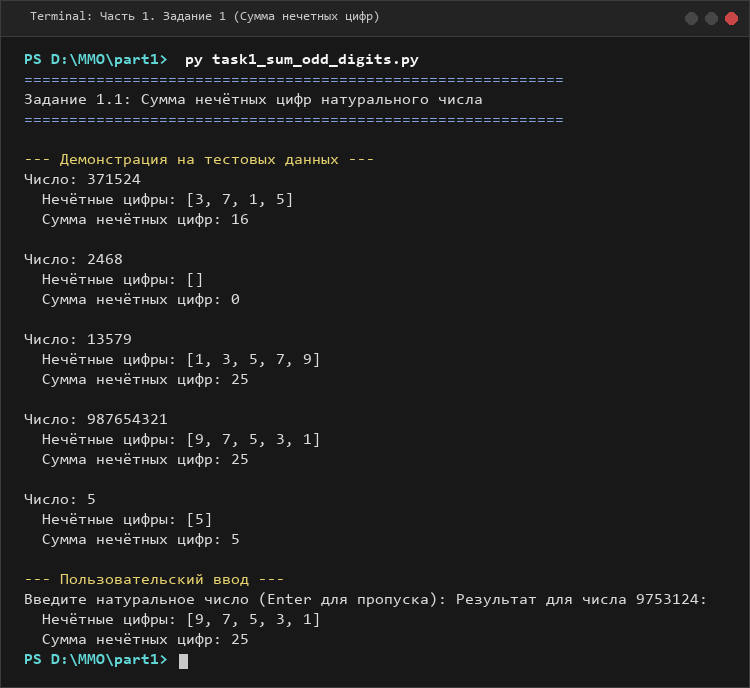
\includegraphics[width=0.88\textwidth]{screenshots/p1_t1.png}
\caption{Результат выполнения задания 1.1}
\end{figure}

На рисунке 5.2 продемонстрирован результат подсчета пар соседних букв верхнего и нижнего регистров, а также согласных букв для слова 'HjkLM' и других тестовых строк.

\begin{figure}[htbp]
\centering
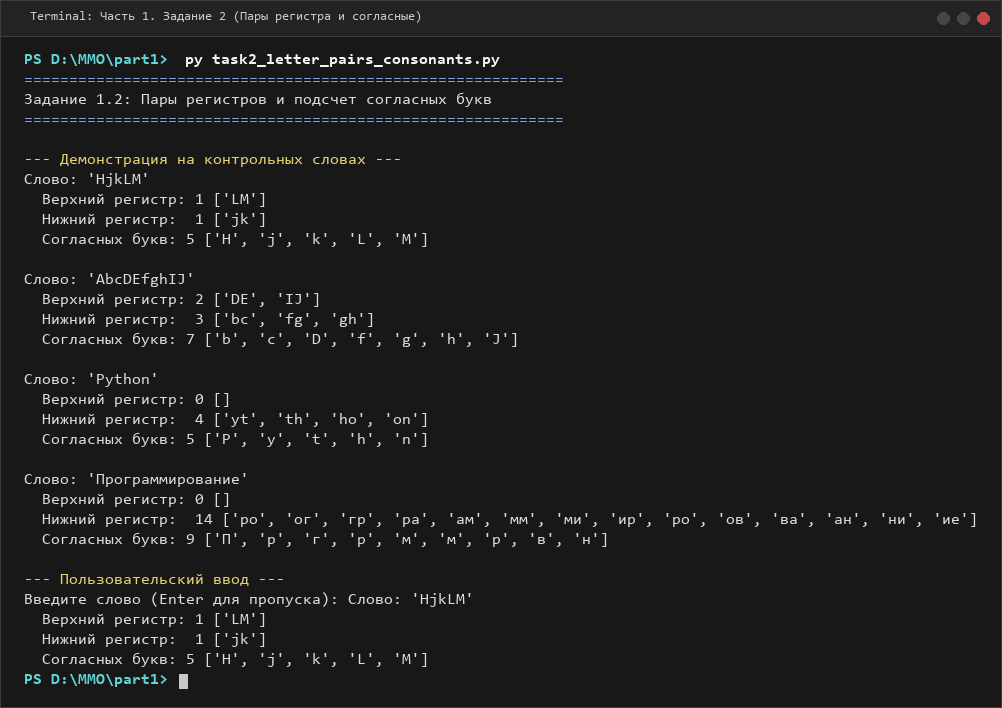
\includegraphics[width=0.88\textwidth]{screenshots/p1_t2.png}
\caption{Результат выполнения задания 1.2}
\end{figure}

На рисунке 5.3 приведен результат обработки списка: замена нечетных чисел на 1, вычисление суммы цифр четных чисел и подсчет гласных и согласных букв в словах.

\begin{figure}[htbp]
\centering
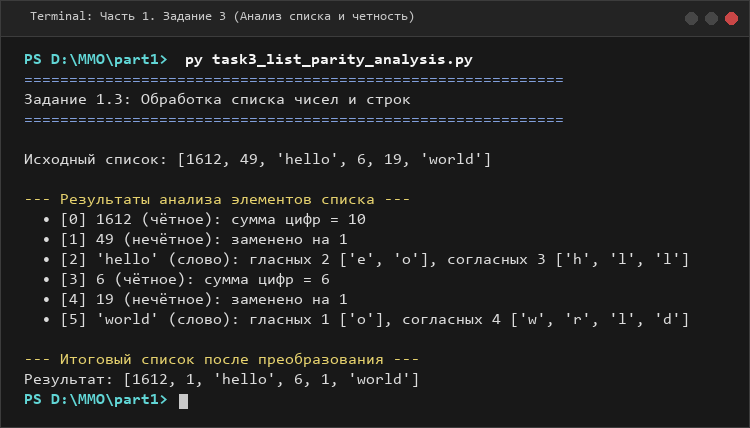
\includegraphics[width=0.88\textwidth]{screenshots/p1_t3.png}
\caption{Результат выполнения задания 1.3}
\end{figure}

На рисунке 5.4 продемонстрирована сортировка словаря по значениям в порядке возрастания и убывания.

\begin{figure}[htbp]
\centering
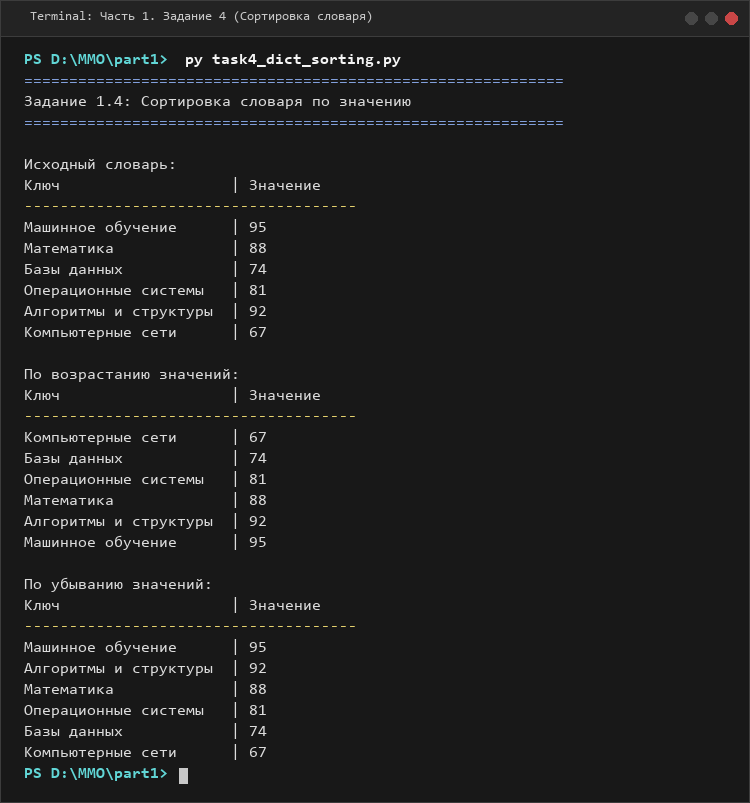
\includegraphics[width=0.88\textwidth]{screenshots/p1_t4.png}
\caption{Результат выполнения задания 1.4}
\end{figure}

На рисунках 5.5 и 5.6 отображена работа программы «Кондитерская»: просмотр полного ассортимента продукции (рисунок 5.5) и процесс покупки с вычислением стоимости чека и выводом остатков (рисунок 5.6).

\begin{figure}[htbp]
\centering
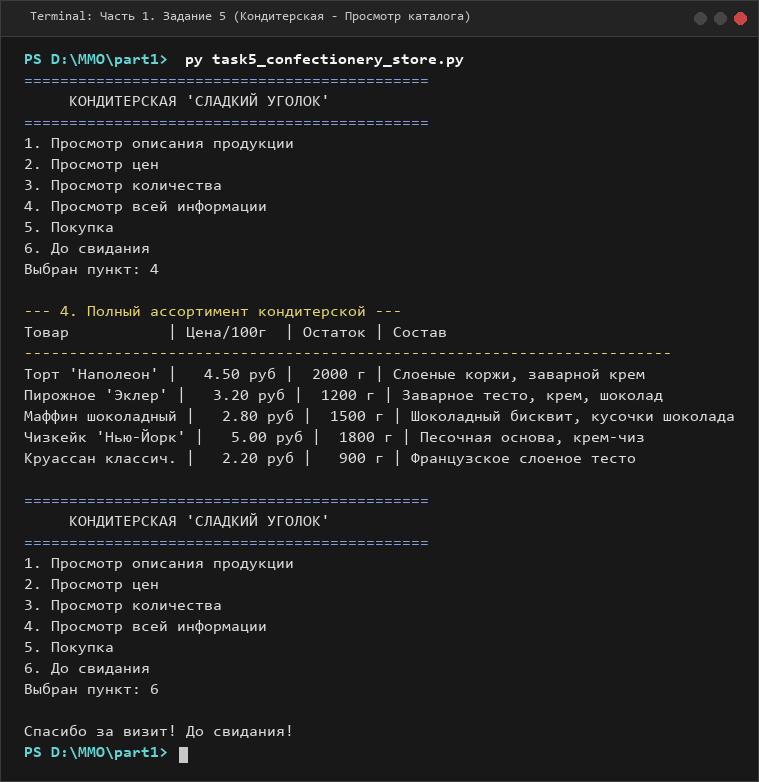
\includegraphics[width=0.88\textwidth]{screenshots/p1_t5_catalog.png}
\caption{Каталог продукции программы «Кондитерская»}
\end{figure}

\begin{figure}[htbp]
\centering
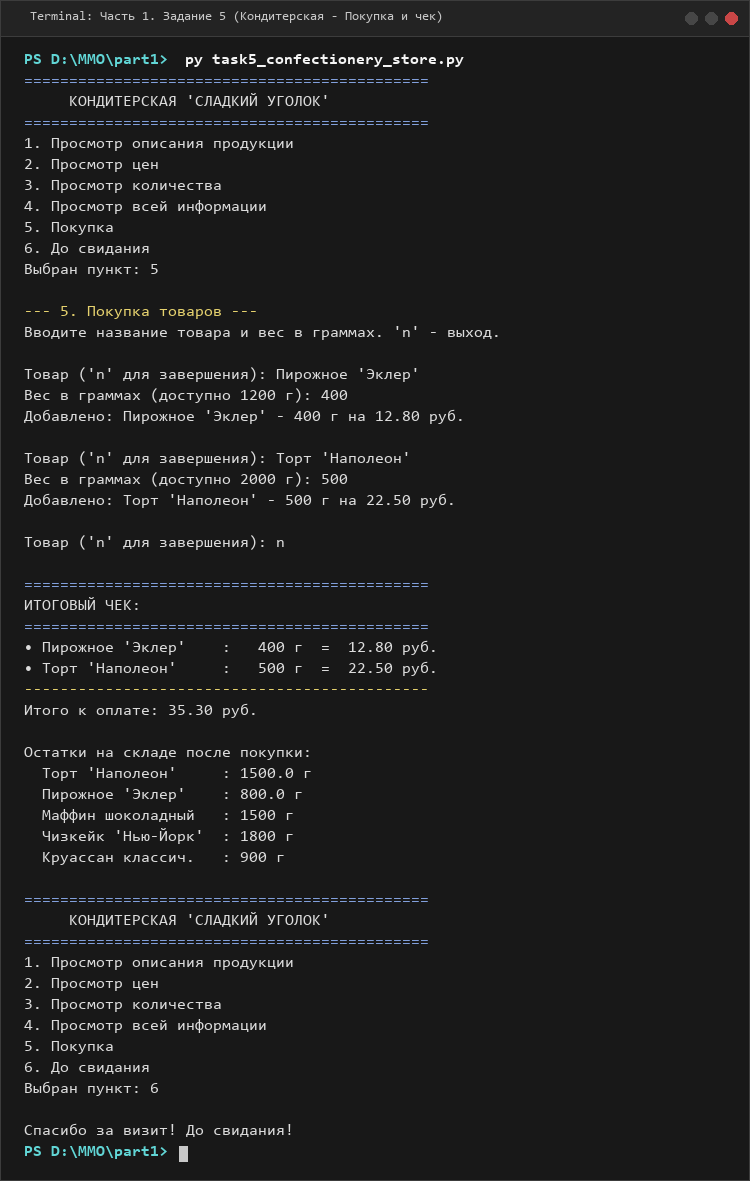
\includegraphics[width=0.88\textwidth]{screenshots/p1_t5_purchase.png}
\caption{Оформление покупки и итоговый чек}
\end{figure}

На рисунке 5.7 показана сортировка кортежа целых чисел по убыванию и вывод его первого и последнего элементов.

\begin{figure}[htbp]
\centering
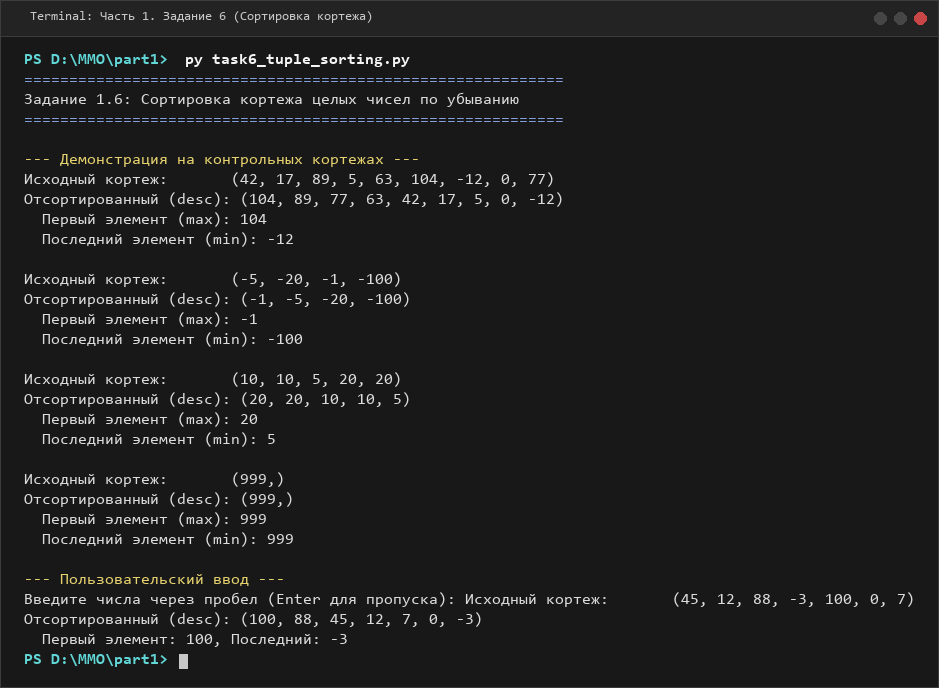
\includegraphics[width=0.88\textwidth]{screenshots/p1_t6.png}
\caption{Результат выполнения задания 1.6}
\end{figure}

\subsection{Результаты выполнения заданий Части 2}

На рисунке 5.8 представлено тестирование функции is\_password\_good на различных наборах паролей с фиксацией результатов в обязательном блоке finally.

\begin{figure}[htbp]
\centering
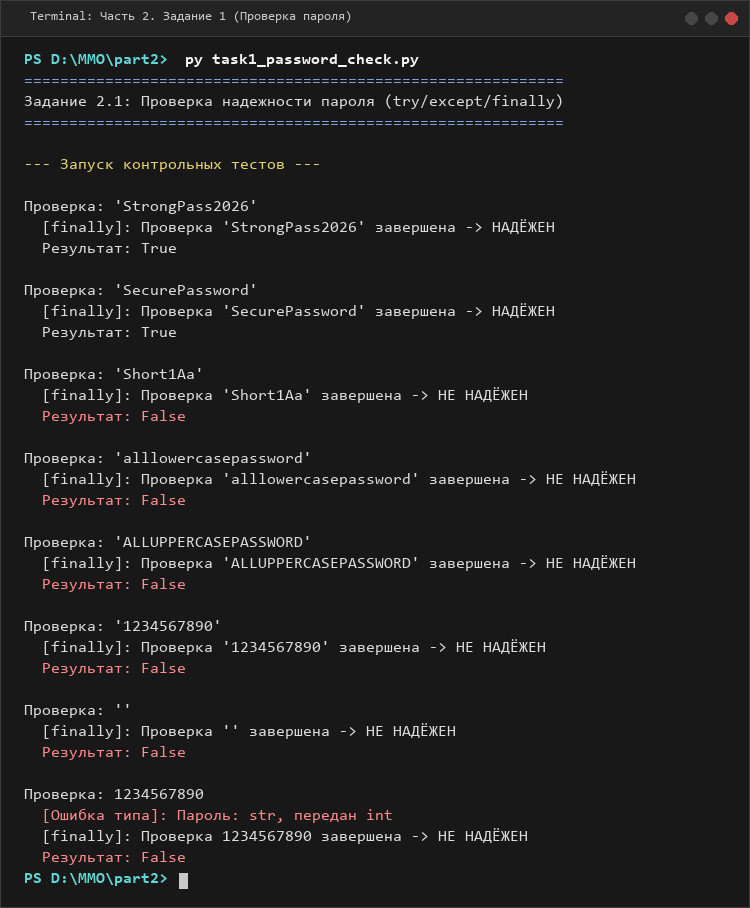
\includegraphics[width=0.88\textwidth]{screenshots/p2_t1.png}
\caption{Тестирование функции is\_password\_good}
\end{figure}

На рисунке 5.9 приведен результат работы универсальной функции обработки кортежа, списка, чисел и строки с перехватом неподдерживаемого типа в блоке try...except.

\begin{figure}[htbp]
\centering
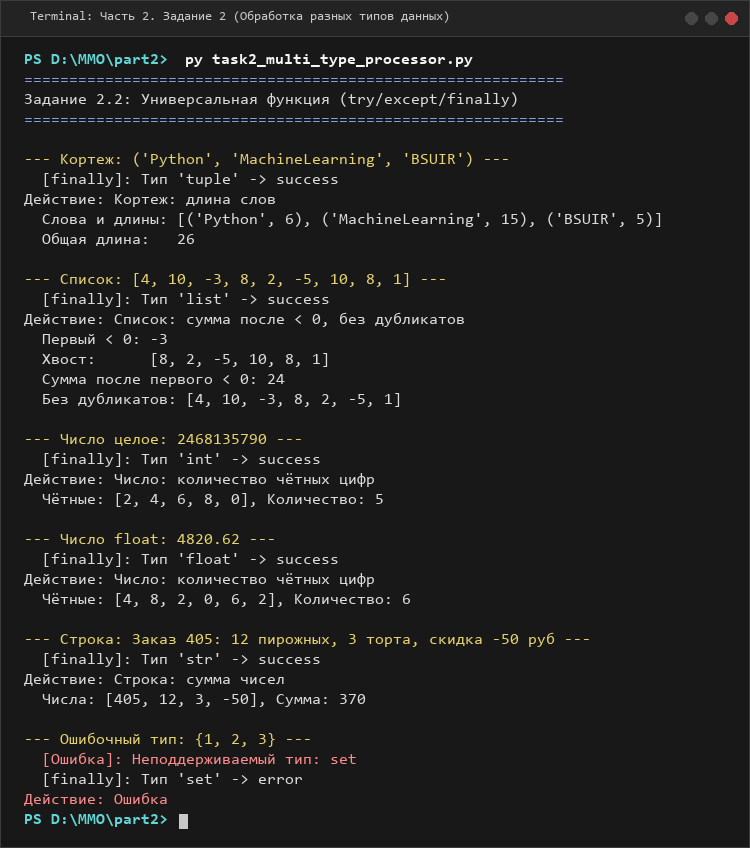
\includegraphics[width=0.88\textwidth]{screenshots/p2_t2.png}
\caption{Обработка различных типов данных}
\end{figure}

На рисунке 5.10 показана работа функции перестановки столбцов матрицы и перехват ошибки выхода индекса за пределы диапазона.

\begin{figure}[htbp]
\centering
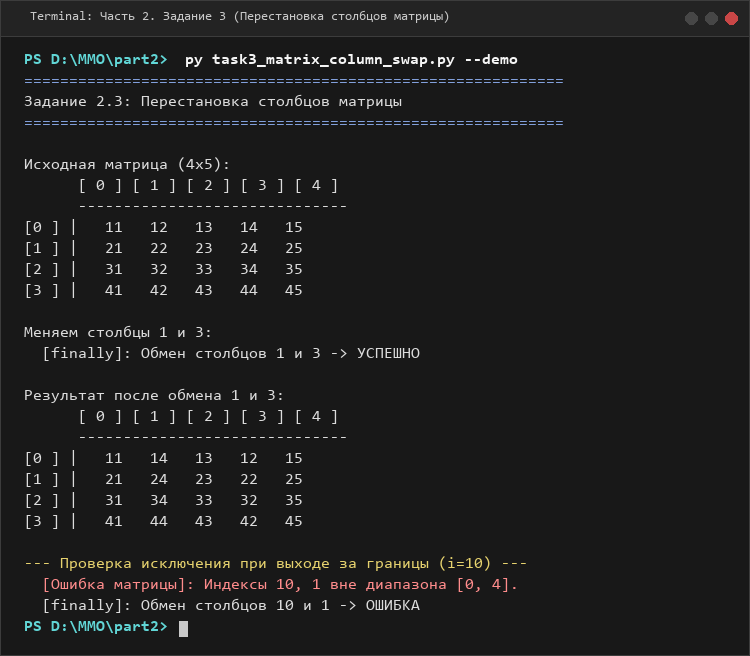
\includegraphics[width=0.88\textwidth]{screenshots/p2_t3.png}
\caption{Перестановка столбцов двумерного массива}
\end{figure}

На рисунке 5.11 продемонстрирована работа конструкции try / except / else / finally при делении чисел, вызове пользовательского исключения и попытке открытия файла.

\begin{figure}[htbp]
\centering
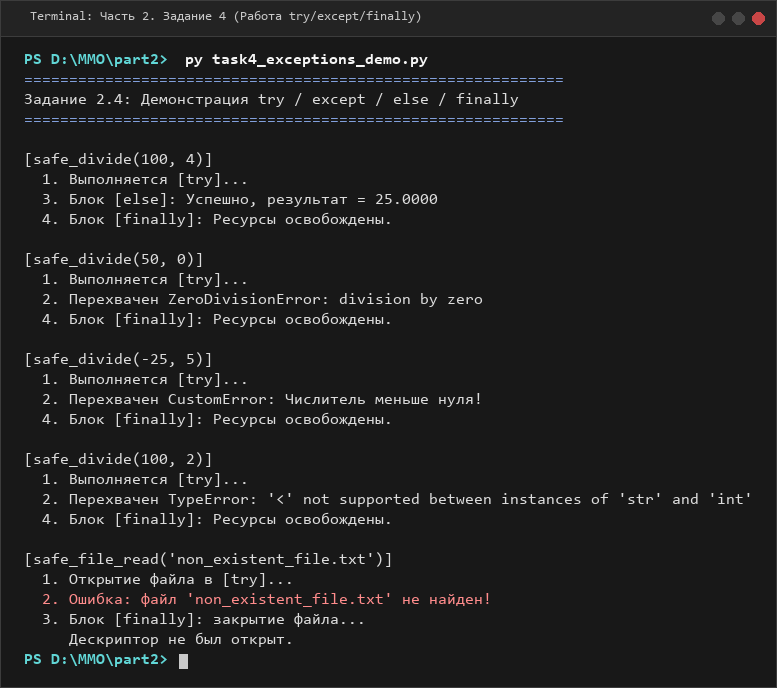
\includegraphics[width=0.88\textwidth]{screenshots/p2_t4.png}
\caption{Демонстрация работы try / except / else / finally}
\end{figure}

\subsection{Результаты выполнения заданий Части 3}

На рисунке 5.12 отображена работа разработанного класса CustomList (добавление, удаление, реверс, сортировка, min/max, уникальные элементы, фильтрация, подсчет частот).

\begin{figure}[htbp]
\centering
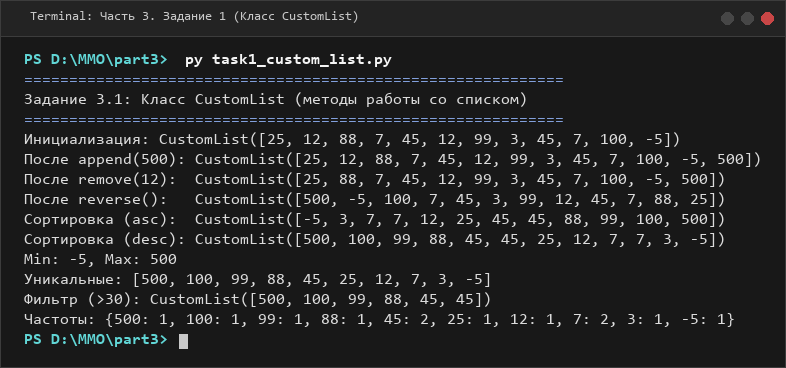
\includegraphics[width=0.88\textwidth]{screenshots/p3_t1.png}
\caption{Работа с классом CustomList}
\end{figure}

На рисунке 5.13 представлен расчет времени и стоимости поездок для классов Самолёт, Поезд, Автомобиль по различным маршрутам, автоматический выбор быстрейшей и экономичной поездки и сохранение отчета в файл.

\begin{figure}[htbp]
\centering
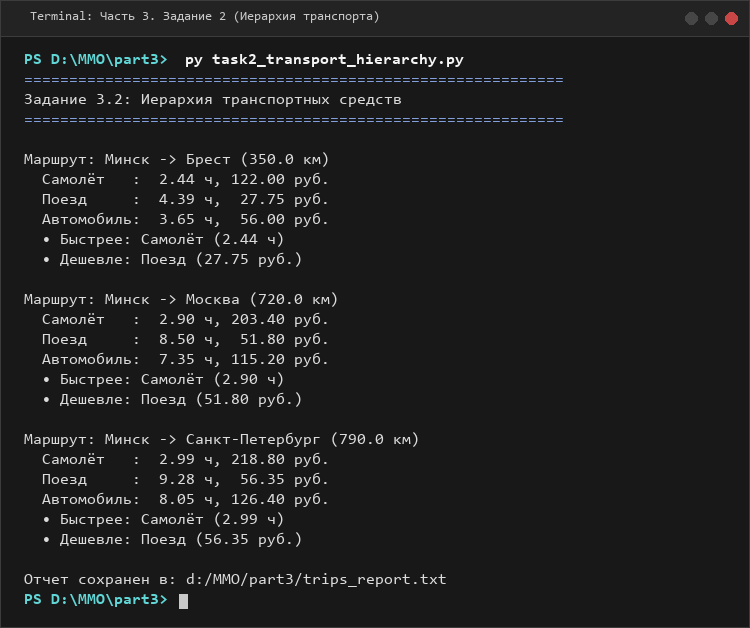
\includegraphics[width=0.88\textwidth]{screenshots/p3_t2.png}
\caption{Иерархия классов транспортных средств}
\end{figure}

На рисунке 5.14 приведен результат работы системы библиотеки: добавление, изменение названия, удаление книг, проверка свойств и экспорт каталога в текстовый файл.

\begin{figure}[htbp]
\centering
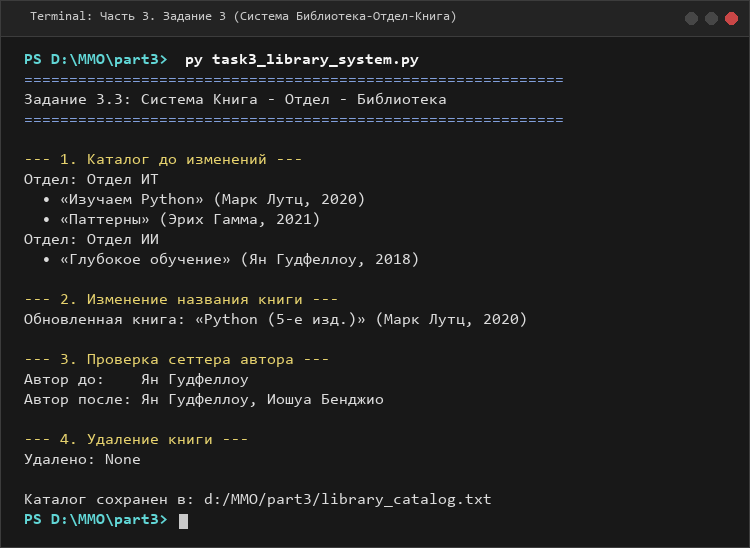
\includegraphics[width=0.88\textwidth]{screenshots/p3_t3.png}
\caption{Система управления библиотекой}
\end{figure}

На рисунке 5.15 показана работа класса StudentAccount с методами экземпляра, методами класса (@classmethod from\_string, get\_honor\_students) и статическими методами-утилитами (@staticmethod validate\_student\_id, convert\_grade\_to\_ects).

\begin{figure}[htbp]
\centering
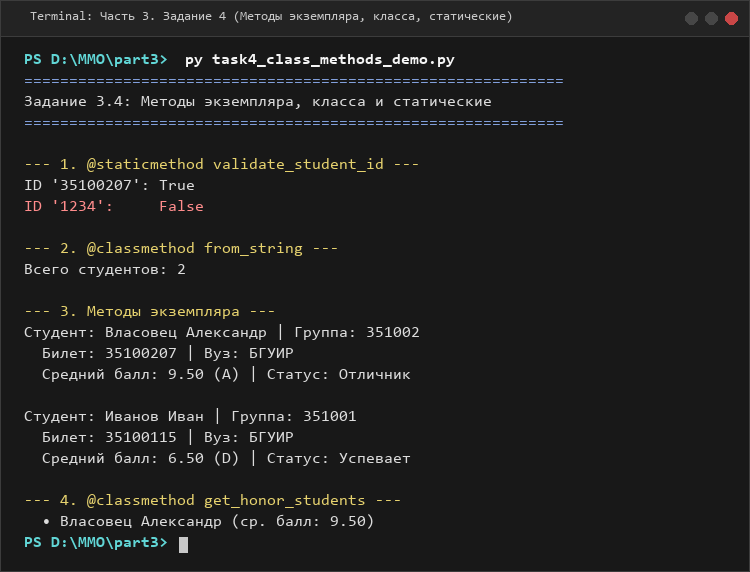
\includegraphics[width=0.88\textwidth]{screenshots/p3_t4.png}
\caption{Методы экземпляра, класса и статические методы}
\end{figure}

% =========================================================================
% 6 ВЫВОДЫ
% =========================================================================
\section{ВЫВОДЫ}

В ходе выполнения комплексной лабораторной работы по дисциплине «Методы машинного обучения» были всесторонне изучены и практически закреплены ключевые аспекты программирования на языке Python. При выполнении начального раздела работы были освоены базовые типы данных, арифметические операции и конструкции управления потоком выполнения. Разработаны алгоритмы нахождения суммы нечетных цифр натурального числа, контекстного анализа регистра смежных символов и подсчета согласных букв. Были изучены операции над гетерогенными динамическими списками, сортировка словарей по значению в прямом и обратном порядке, а также сортировка неизменяемых кортежей с извлечением экстремальных значений. Спроектированная интерактивная программа управления ассортиментом кондитерской наглядно продемонстрировала эффективное применение словарей со сложной структурой значений для хранения характеристик продукции, обработки пользовательских заказов и пересчета складских остатков.

Второй этап исследований позволил освоить принципы модульной декомпозиции алгоритмов и построения отказоустойчивого программного обеспечения. Реализованная функция валидации паролей обеспечила надежную проверку критериев безопасности с протоколированием статуса завершения в блоке finally. Разработанный универсальный обработчик структур данных продемонстрировал корректное ветвление логики в зависимости от динамического типа входного аргумента, включая вычисление длины строк кортежа, суммирование элементов списка после первого отрицательного значения с удалением дубликатов, подсчет четных разрядов чисел и парсинг числовых подстрок. Алгоритм поэлементного обмена столбцов матрицы подтвердил практические навыки манипуляции двумерными массивами. На примере комплексного сценария было доказано преимущество конструкции try / except / else / finally, которая гарантирует корректное освобождение файловых дескрипторов и перехват исключений времени выполнения.

Заключительный этап работы был посвящен практической реализации принципов объектно-ориентированного программирования. Спроектированный класс CustomList предоставил расширенный интерфейс для управления списковыми структурами, включая фильтрацию, частотный анализ и поиск экстремумов. Построенная иерархия классов транспортных средств на базе общего суперкласса обеспечила гибкий полиморфный расчет параметров перевозки по заданным маршрутам, автоматический выбор оптимального по времени и стоимости варианта с экспортом результатов во внешний файл. В информационной системе библиотеки была продемонстрирована строгая инкапсуляция атрибутов с помощью декораторов @property и сеттеров с валидацией данных. Разработанный класс студенческого аккаунта наглядно продемонстрировал четкое функциональное разграничение методов экземпляра, методов класса с фабричным созданием объектов и независимых статических методов-утилит. Все разработанные программы успешно протестированы, а структура отчета полностью соответствует требованиям стандарта СТП 01-2017.

\end{document}
